\subsection{Neural Language Models}
In the computational experiments, we use a Neural Language Model (NLM).
In computational linguistics, a \emph{language model} refers to a model that defines a probability distribution over sequences of words.
The language model that we consider here -- a recurrent LSTM-based language model \citep{Hochreiter:Schmidhuber:1997} -- factorizes this probability into a multiplication of the conditional probabilities of all words in the sentence, given the words that precede them:

\begin{equation}
    P(w_1 w_2 \cdots w_n) = \prod_i p(w_i|w_1 \cdots w_{i-1})
\end{equation}

This type of neural language models can thus be used as \emph{next-word predictors}: given the preamble of a sentence, they output a probability distribution over potential next words.
We exploit this fact in our experiments.

\begin{figure}
    \centering
    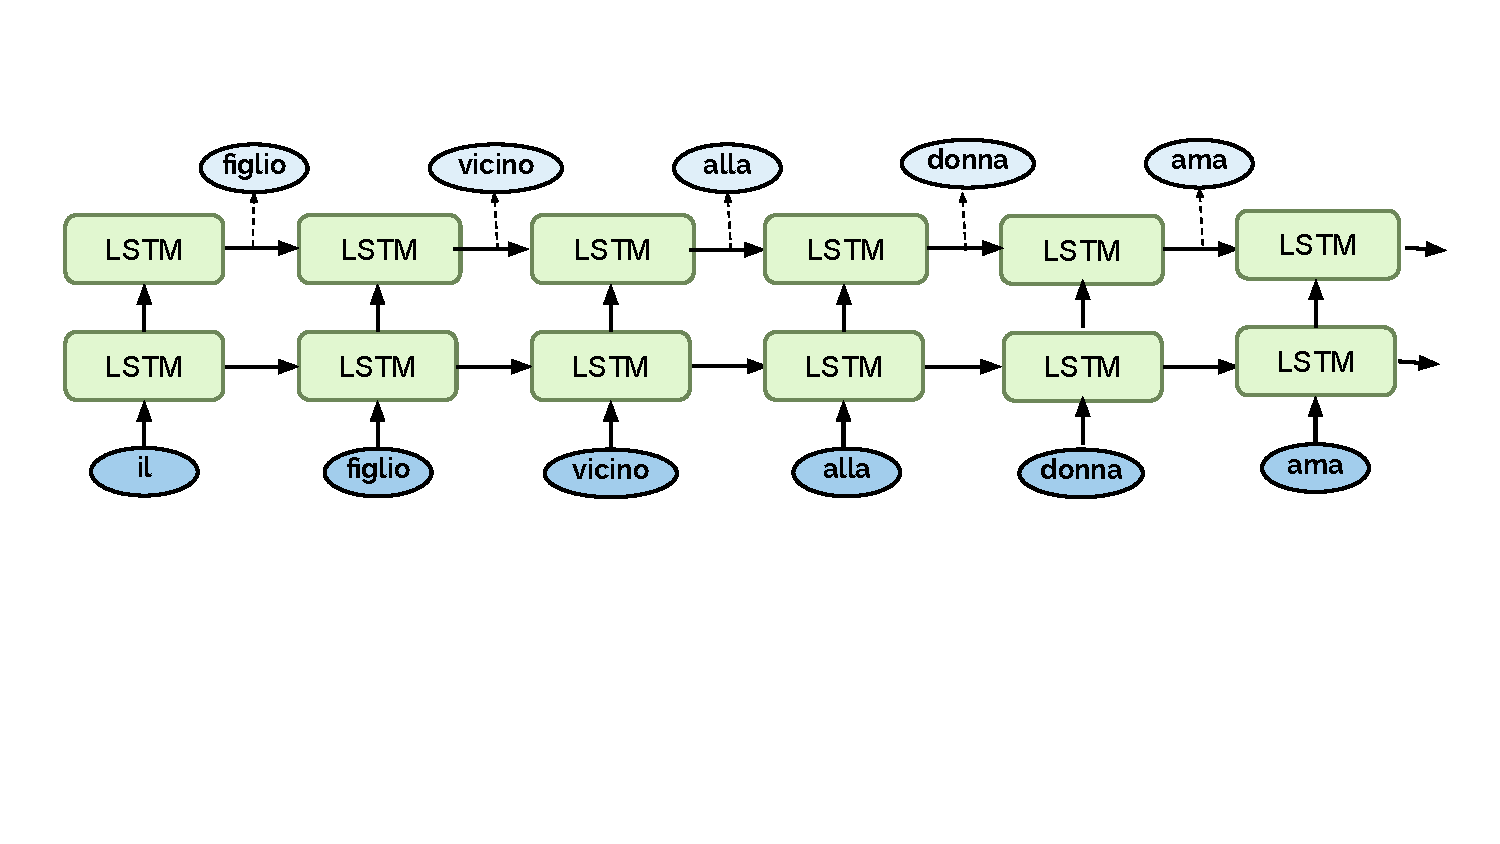
\includegraphics[width=0.8\textwidth, clip, trim={10mm 50mm 10mm 20mm}]{figures/LM-image}
    \caption{Graphical description of a two-layer LSTM language model. At each timestep, the model processes an input word and outputs a probability distribution over potential next words in the sentence. The prediction of the output word depends on both the input word and on the previous state of the model, which serves as a context (horizontal arrows).} 
    %For each presented sentence in our experiments, we do not consider the full probability distribution, but instead compare the probabilities of the two forms of the relevant verb or adjective.}
\end{figure}

\subsubsection{Model Description}
The specific NLM we use in our experiments is the Italian NLM made available by \citet{Gulordava:etal:2018}\footnote{\url{https://github.com/facebookresearch/colorlessgreenRNNs}}.
This model is a recurrent NLM, consisting of two layers, each with 650 Long-Short Term Memory (LSTM) units \citep{Hochreiter:Schmidhuber:1997}, input and output embedding layers of 650 units and input and output layers of size 50000 (the size of the vocabulary). 
The weights of the input and output embedding layers are not shared \citep{press2016using}.
The last layer of the model is a softmax layer, whose activations sum up to 1 and as such corresponds to a probability distribution over all words in the NLM's vocabulary. 

\subsubsection{Model training}
NLMs are typically trained by presenting them with large amounts of data (a \emph{training corpus}) and providing them feedback on how well they can predict it, which allows them to adjust their parameters to maximize the probabilities of the sentences in this corpus.
During model training, they are evaluated by how well they do so, as expressed in the \emph{perplexity} of the training corpus (roughly, the exponent of the average negative log-likelihood of the data).
Our NLM was trained on a sample of the Italian Wikipedia text, containing 80M word tokens and 50K word types. Further details can be found in \citet{Gulordava:etal:2018}.


\subsubsection{Model Evaluation on the Number-Agreement Tasks}
Following \citet{Linzen:etal:2016}, we compute the model's accuracy for the different NA-tasks by considering whether the model prefers the correct verb or adjective form (for the NounPP-number and NounPP-gender tasks, respectively).
We do so by presenting the preamble of each sentence to the NLM and then comparing the output probabilities assigned to the plural and singular forms of the verb for the NounPP task and the probabilities of the masculine and feminine forms for the NounPP-gender task.
On each sentence, the model is scored 1 if the probability of the correct verb is higher than the wrong, and else 0. 
The model's accuracy is then defined as the average of these scores across all sentences in the NA-task. 

\subsubsection{Ablation Experiments}
To identify units that play an important role in the encoding of number and gender, we run a series of ablation tests.
In these ablation tests, we assess the impact of a \emph{single unit} on model performance by setting the activation of the unit to zero and then recomputing the performance of the model on the NounPP-noun and NounPP-gender NA-tasks. 
We conduct such ablation studies for all recurrent units in the network, resulting in 1300 ablation studies per task.

